\documentclass[jou]{apa6}
\usepackage{lmodern}
\usepackage{amssymb,amsmath}
\usepackage{ifxetex,ifluatex}
\usepackage{fixltx2e} % provides \textsubscript
\ifnum 0\ifxetex 1\fi\ifluatex 1\fi=0 % if pdftex
  \usepackage[T1]{fontenc}
  \usepackage[utf8]{inputenc}
\else % if luatex or xelatex
  \ifxetex
    \usepackage{mathspec}
  \else
    \usepackage{fontspec}
  \fi
  \defaultfontfeatures{Ligatures=TeX,Scale=MatchLowercase}
\fi
% use upquote if available, for straight quotes in verbatim environments
\IfFileExists{upquote.sty}{\usepackage{upquote}}{}
% use microtype if available
\IfFileExists{microtype.sty}{%
\usepackage{microtype}
\UseMicrotypeSet[protrusion]{basicmath} % disable protrusion for tt fonts
}{}
\usepackage{hyperref}
\hypersetup{unicode=true,
            pdftitle={How Many Psychologists Use Questionable Research Practices? Estimating the Population Size of Current QRP Users},
            pdfauthor={Nicholas W. Fox, Nathan Honeycutt, \& Lee Jussim},
            pdfkeywords={QRPs, Questionable Research Practices, Replication Crisis, Social
Networks},
            pdfborder={0 0 0},
            breaklinks=true}
\urlstyle{same}  % don't use monospace font for urls
\usepackage{graphicx,grffile}
\makeatletter
\def\maxwidth{\ifdim\Gin@nat@width>\linewidth\linewidth\else\Gin@nat@width\fi}
\def\maxheight{\ifdim\Gin@nat@height>\textheight\textheight\else\Gin@nat@height\fi}
\makeatother
% Scale images if necessary, so that they will not overflow the page
% margins by default, and it is still possible to overwrite the defaults
% using explicit options in \includegraphics[width, height, ...]{}
\setkeys{Gin}{width=\maxwidth,height=\maxheight,keepaspectratio}
\IfFileExists{parskip.sty}{%
\usepackage{parskip}
}{% else
\setlength{\parindent}{0pt}
\setlength{\parskip}{6pt plus 2pt minus 1pt}
}
\setlength{\emergencystretch}{3em}  % prevent overfull lines
\providecommand{\tightlist}{%
  \setlength{\itemsep}{0pt}\setlength{\parskip}{0pt}}
\setcounter{secnumdepth}{0}
% Redefines (sub)paragraphs to behave more like sections
\ifx\paragraph\undefined\else
\let\oldparagraph\paragraph
\renewcommand{\paragraph}[1]{\oldparagraph{#1}\mbox{}}
\fi
\ifx\subparagraph\undefined\else
\let\oldsubparagraph\subparagraph
\renewcommand{\subparagraph}[1]{\oldsubparagraph{#1}\mbox{}}
\fi

%%% Use protect on footnotes to avoid problems with footnotes in titles
\let\rmarkdownfootnote\footnote%
\def\footnote{\protect\rmarkdownfootnote}


  \title{How Many Psychologists Use Questionable Research Practices? Estimating
the Population Size of Current QRP Users}
    \author{Nicholas W. Fox\textsuperscript{1}, Nathan Honeycutt\textsuperscript{1},
\& Lee Jussim\textsuperscript{1}}
    \date{}
  
\shorttitle{How Many Psychologists Use QRPs}
\affiliation{
\vspace{0.5cm}
\textsuperscript{1} Rutgers University}
\keywords{QRPs, Questionable Research Practices, Replication Crisis, Social Networks\newline\indent Word count: 4,492}
\usepackage{csquotes}
\usepackage{upgreek}
\captionsetup{font=singlespacing,justification=justified}

\usepackage{longtable}
\usepackage{lscape}
\usepackage{multirow}
\usepackage{tabularx}
\usepackage[flushleft]{threeparttable}
\usepackage{threeparttablex}

\newenvironment{lltable}{\begin{landscape}\begin{center}\begin{ThreePartTable}}{\end{ThreePartTable}\end{center}\end{landscape}}

\makeatletter
\newcommand\LastLTentrywidth{1em}
\newlength\longtablewidth
\setlength{\longtablewidth}{1in}
\newcommand{\getlongtablewidth}{\begingroup \ifcsname LT@\roman{LT@tables}\endcsname \global\longtablewidth=0pt \renewcommand{\LT@entry}[2]{\global\advance\longtablewidth by ##2\relax\gdef\LastLTentrywidth{##2}}\@nameuse{LT@\roman{LT@tables}} \fi \endgroup}



\authornote{Department of Psychology, Rutgers University,
Piscataway NJ 08854. Open for construtive comments Aug 14th - Aug 21
2018, prior to submission for publication. Data and materials:
\url{https://osf.io/2zwqf}

Correspondence concerning this article should be addressed to Nicholas
W. Fox, 53 Avenue E, Room 429, Piscataway NJ 08854. E-mail:
\href{mailto:nwf7@psych.rutgers.edu}{\nolinkurl{nwf7@psych.rutgers.edu}}}

\abstract{
Psychology has been in crisis. Over the past 15 years many high-impact
research findings have failed to replicate, calling into question their
validity. Increased methodological and statistical scrutiny has led to
field-wide introspection on how best to produce robust, reproducible,
research. One focus has been on the use of questionable research
practices. Previous estimates of the number of researchers who use
questionable research practices vary widely, from over 60\% to near
10\%. In the current work, the authors produced three estimates of the
number of American psychologists who have used questionable research
practices in the last 12 months, utilizing direct, indirect, and social
network measures of estimation. We estimate up to 24.40`\% of American
psychologists have recently used at least one questionable research
practice. These estimates represent the first step in generating
actionable interventions to resolve the current replication crisis and
increase trust in published research.


}

\usepackage{amsthm}
\newtheorem{theorem}{Theorem}[section]
\newtheorem{lemma}{Lemma}[section]
\theoremstyle{definition}
\newtheorem{definition}{Definition}[section]
\newtheorem{corollary}{Corollary}[section]
\newtheorem{proposition}{Proposition}[section]
\theoremstyle{definition}
\newtheorem{example}{Example}[section]
\theoremstyle{definition}
\newtheorem{exercise}{Exercise}[section]
\theoremstyle{remark}
\newtheorem*{remark}{Remark}
\newtheorem*{solution}{Solution}
\begin{document}
\maketitle

It is the researcher's job to generate theories, test hypotheses,
collect and interpret data, interpret results, and to publish findings.
This is all done to learn more about the world and how it works. In the
course of doing science, the researcher has many decisions to make: How
many subjects will I use? How will I operationalize my variables? What
is my population of interest? Should I exclude any data from the
analysis?

Each decision point is a \enquote{researcher degree of freedom}
(Simmons, Nelson, \& Simonsohn, 2011), with the potential of introducing
error and bias. Since there is a high level of ambiguity in research,
these degrees of freedom can be resolved in different ways. In reviewing
how researchers deal with outlying observations, Simmons et al. (2011)
found different research groups made independent decisions on the best
course of action. When researchers cleaned data and removed participants
that responded \enquote{too fast}, some defined this as 2 standard
deviations below the mean response speed, some defined it as
observations below 200ms, and others removed the fastest 2.5\% of
respondents. None of these definitions are inherently an incorrect
interpretation of \enquote{too fast}, which can be a problem: without
clear standards in place, this type of flexible decision making can blur
the lines between what decision is right, what decision produces the
desired result, and what decision is most likely to help get a finding
published.

There are many \enquote{degrees of freedom} that exploit the gray areas
of acceptable practice that may bias research findings (John,
Loewenstein, \& Prelec, 2012; Wicherts et al., 2016). Some examples
include trying different ways to score the chosen primary dependent
variable, and deciding how to deal with outliers in an ad hoc manner.
Ten of these behaviors have been collectively called
\enquote{questionable research practices} (QRPs) and are typically
defined as behaviors during data collection, analysis, and reporting
that have the potential to increase false-positive findings in the
literature. While there are many examples of other behaviors that could
be considered questionable, these ten stand out as being familiar to
most researchers and having been investigated previously (Agnoli,
Wicherts, Veldkamp, Albiero, \& Cubelli, 2017; Fiedler \& Schwarz, 2016;
John et al., 2012). For this study, nine of the ten QRPs were considered
(Table \ref{tab:QRPs}). We did not include \enquote{fabricated data}
(QRP-10) as a questionable research practice as the authors consider
this a fraudulent, not questionable, behavior. Not only can QRP use
increase the number of false-positive findings (e.g., taking a
\enquote{non-significant} result and pushing it over a threshold into
being \enquote{significant}), but using multiple QRPs can also influence
the reported effect size of a given finding due to sampling bias and low
power (Button et al., 2013). Thus, QRP use could lead to field-wide
interpretations that are not warranted by the data.

\begin{table*}

\caption{\label{tab:QRPs}Questionable Research Practices of interest with examples.}
\centering
\fontsize{9}{11}\selectfont
\begin{tabular}[t]{l>{\raggedright\arraybackslash}p{20em}>{\raggedright\arraybackslash}p{20em}}
\toprule
Item & Questionable Research Practice & Example\\
\midrule
1 & Failing to report all of a study's dependent measures & After measuring baseline anxiety with three different scales, only reporting one\\
2 & Collecting more data after looking to see if the results were significant & Collecting 25 subjects' worth of data, achieving p = 0.07, then recruiting 25 more subjects\\
3 & Failing to report all of a study's conditions & Collecting data on three experimental conditions (no/low/high anxiety), but only reporting two (no/high anxiety)\\
4 & Stopping data collection earlier than planned because one found the result one was looking for & After collecting half the final number of proposed subjects, achieving p < 0.05, then stopping recruitment\\
5 & Rounding off p values to achieve significance & Achieving p = 0.054, then reporting it as p = 0.05 or p < 0.05\\
\addlinespace
6 & Selectively reporting studies that 'worked' & Running eight studies, but only reporting the 5 that had significant findings\\
7 & Deciding whether to exclude observations after seeing the effect of doing so on the results & Removing potential outliers based on their effect on the data and no on an a priori guideline\\
8 & Reporting unexpected findings as being predicted from the start (a.k.a Hypothesizing After the Results are Known, or HARKing) & Predicting a relationship between A and B, but finding a relationship between A and C, reporting the A-C relationship was predicted from the start\\
9 & Reporting results are unaffected by demographics when actually unsure or not tested & Reporting no gender differences when gender was not collected or relationship not tested\\
\bottomrule
\end{tabular}
\end{table*}

\subsection{Prevalence of questionable research
practices}\label{prevalence-of-questionable-research-practices}

Consider one of the most basic questions to ask about the current
replication crisis: How many people are contributing to it? John et al.
(2012) found 63\% of psychologists admitted to publishing work without
all the dependent measures included (at some point in their academic
career). As articulated by Simmons et al. (2011), this is highly
problematic because increasing the number of dependent variables is
correlated with an increase in the probability of finding a significant
result. Without reporting all dependent measures, readers are left with
a false impression of the rarity or truthfulness of the reported
findings. But, this estimate from John et al. (2012) was contested by
Fiedler and Schwarz (2016). In their conceptual replication that used
differently worded questions, used a different conceptualization of
\enquote{prevalence}, and tested a German (as opposed to an American)
cohort of psychologists, Fiedler and Schwarz (2016) found less than 10\%
prevalence of the same questionable practice (omitting dependent
variables). Furthermore, Agnoli et al. (2017) recently replicated the
original John et al. (2012) study in an Italian cohort of psychologists,
and found similarly high levels of QRP use (47.9\% of respondents had
omitted dependent variables). Concequently, there is no current
consensus on the prevalence of QRP use in psychology, nor any indication
of how these may be related to the current replication crisis in the
field.

Given the inconsistencies in assessing the prevalence of QRP use, the
present work sought to expand on this existing literature in several
ways. First, we investigated current QRP users, operationalized as a
person who has used at least one of nine QRPs \enquote{in the past 12
months}. This puts QRP use into the timeframe of the current replication
crisis. Second, it addressed the larger issue of \enquote{prevalence},
by defining behaviors performed within a specified time period. Previous
work estimating QRP prevalence has done so over career-long timespans or
via estimating frequency of QRP use, both providing limited insight on
the current issues in the field.

A third unique contribution of the present research is that it assessed
prevalence of QRP use with three starkly different methodologies. One
was a direct estimate tightly based on prior research (i.e., (Agnoli et
al., 2017; Fiedler \& Schwarz, 2016; John et al., 2012)): We simply
asked researchers to report their own QRP use.

However, two other methods were increasingly different from this
straightforward assessment. One used the unmatched count technique, an
indirect estimate aimed at reducing social desirability response bias
((Arentoft et al., 2016) - see Method for details). The second generated
an indirect estimate of QRP use by using social network information from
the general population of psychologists (Jing, Qu, Yu, Wang, \& Cui,
2014; M. J. Salganik et al., 2011; Zhang et al., 2010; Zheng, Salganik,
\& Gelman, 2006). Neither the unmatched count technique nor this social
network method required participants to identify as belonging to a
potentially stigmatized group (i.e., QRP users), thereby reducing the
risk of socially desirable response bias compared to more traditional
direct estimates. While network methods were expected to provide
insights into QRP use prevalence, they have yet to be used in
psychology. Thus, this work produced three estimates of QRP use
prevalence.

\section{METHOD}\label{method}

The work detailed in this manuscript was preregistered on May 15th,
2017. The preregistration can be found at www.osf.io/xu25n. For
additional details, and descriptions of the minor deviations from the
preregistration, see the supplemental materials.

\subsection{Sample}\label{sample}

The population of interest was tenured or tenure-track faculty
associated with a psychology department at a PhD-granting institution in
the United States. The population contained 7,101 individuals as of June
2017. All 7,101 members of this population were contacted via email and
asked to participate. Of the 7,101 email invitations sent, 214 emails
bounced (3.01\%). We collected 613 full responses (8.63\% full response
rate), and 296 partial responses. Only full responses are used in the
following estimations. Additionally, 26 participant responses were
removed for either being marked complete erroneously or due to breaking
estimate-specific criteria. There was no compensation offered for
participation. 299 (48.78\%) participants identified as female, 279
(45.51\%) identified as male, and 19 (3.10\%) chose not to identify
their gender. 131 (21.37\%) participants identified as an Assistant
Professor, 141 (23.00\%) as Associate Professor, and 208 (33.93\%) as
Full Professor. 113 participants identified as tenure or tenure-track,
but did not disclose their tenure level.

\subsection{Data Sources}\label{data-sources}

Data was collected using three surveys, designed and distributed using
Qualtrics survey software (Qualtrics, 2005). Each survey asked questions
designed to estimate the total social network size of the participant,
as well as demographic questions. Surveys 1 and 2 each contained
questions appropriate for the unmatched count technique (UCT). Survey 3
contained, instead of the UCT, our direct estimate measure and questions
used to determine transmission of QRP-identity information within an
individual's social network.

Participants were contacted by email and provided a link to one of the
Qualtrics surveys. Upon agreeing to the informed consent, participants
completed the aforementioned measures. To ensure the highest number of
participants in our game of contacts procedure (see Measures), half of
the total population were asked to participate in Survey 3, which
contained our direct estimate question. Thus, 3551 were solicited for
Survey 3. The remaining 3550 psychologists contacted were asked to
participate in our unmatched count estimate (Survey 1 or Survey 2), with
1775 randomized into the innocuous list group, and 1775 randomized into
the concealable list group. Participants had seven days to complete the
survey upon starting. Since data was collected between September 2017
and December 2017, questions framed \enquote{in the past 12 months}
bound actual QRP use between September 2016 and December 2017, a time
frame of 15 months. Therefore, estimates of \enquote{current QRP use}
are based on the number of psychologists who have used at least one QRP
in this time frame.

All surveys included the definition of \enquote{Questionable Research
Practices (QRPs)}. This definition included the list of behaviors
previously defined in the literature as QRPs (see Table \ref{tab:QRPs}),
but omitting \enquote{fabricating data} for reasons addressed earlier.
The definition of QRP was made available on each relevant question with
a mouse rollover that was first demonstrated with the initial
definition. For the full text of our definition used, see supplemental
materials.

Additionally, QRP use (as defined in the present work) is constrained to
behaviors performed \enquote{in the past 12 months}. Although some have
found instances of underreporting when using a 12 month recall (Connelly
\& Brown, 1995; Landen \& Hendricks, 1995), this time frame is used
frequently to measure current behavior in major national data collection
surveys such as the National Health Interview Survey (NHIS) (United
States Census Bureau, 2018) and the National Survey on Drug Use and
Health (Ahrnsbrak, Bose, Hedden, Lipari, \& Park-Lee, 2017).

\subsection{Measures}\label{measures}

\subsubsection{Direct Estimate}\label{direct-estimate}

The direct estimate involved asking members of the target population
whether they have used at least one QRP in the past 12 months, and is
calculated as follows:

\begin{equation}
\rho = \frac{c}{n}
\end{equation}

where \(\rho\) is the proportion estimate of people who have used at
least one QRP in the past 12 months, \(c\) is the number of participants
indicating they have used a QRP in the past 12 months, and \(n\) is the
total number of participant responses.

\subsubsection{Unmatched Count
Technique}\label{unmatched-count-technique}

The unmatched count technique (UCT) is an indirect way of measuring the
base rates of concealable and potentially stigmatized identities
(Gervais \& Najle, 2017; Wolter \& Laier, 2014). In this estimate, two
groups of participants are given a list of innocuous items that could
apply to them (e.g., I own a dishwasher; I exercise regularly). The list
of items for both groups is the same except for one additional item that
one group receives and the other does not. This extra item asks about
the concealable identity (e.g., I own a dishwasher; I exercise
regularly; I smoke crack cocaine - examples from (Gervais \& Najle,
2017)). See Table \ref{tab:UCT} for the full list of items used.
Participants are asked to count and report the number of items in the
list that apply to them. At no point does a participant identify
themselves with any particular list item, only the total number of
applicable items. The proportion of participants that identify with the
stigmatized identity is calculated as:

\begin{equation}
\rho = \frac{\sum x_y^s}{n^s} - \frac{\sum x_y^i}{n^i}
\end{equation}

where \(\rho\) is the proportion estimate of people who have used at
least one QRP in the past 12 months, \(x_y^s\) is the number of reported
items for participant \(y\) in the sensitive list group \(s\), \(n^s\)
is the total number of participant responses in group \(s\), \(x_y^i\)
is the number of reported items for participant \(y\) in the innocuous
list group \(i\), and \(n^i\) is the total number of participants in
group \(i\).

\subsubsection{Generalized Network Scale-Up
Method}\label{generalized-network-scale-up-method}

Network methods estimate population sizes using information about the
personal networks (referred to as \enquote{ego networks} in this
literature, i.e., (McCormick, Salganik, \& Zheng, 2010)) of respondents,
based on the assumption that personal networks are, on average,
representative of the population (M. J. Salganik et al., 2011). Each
participant's social network provides a sample of the general
population, and by collecting network data on many participants, those
accumulated social networks provide access to the larger population.

Participants were asked about how many people they \enquote{know} in the
population of interest. In this study, \enquote{know} was defined as:
they know you by face or by name, you know them by face or by name, you
could contact the person if you wanted to, and you've been in contact in
the past two years (H. R. Bernard et al., 2010). Participants were then
asked a series of questions to estimate the total size of their social
network, and the number of people they know who have used at least one
QRP in the past 12 months. Together, the network scale-up can be used to
estimate the proportion of QRP users, and was calculated as follows:

\begin{equation}
\rho = \frac{\sum y_i}{\sum d_i}
\end{equation}

where \(\rho\) is the proportion estimate of people who have used at
least one QRP in the past 12 months, \(y_i\) is the number of people
known in the target group \(y\) by participant \(i\), and \(d_i\) is the
estimated total number of people known \(d\) by participant \(i\) within
the population of interest (see Killworth, McCarty, Bernard, Shelley,
and Johnsen (1998) for more on estimating \(d\)). Equation 3 makes two
assumptions: that members of the population of interest know all
identity information about all members of their ego networks, and that
QRP users have the same size social networks as the general population
of interest.

\begin{table}

\caption{\label{tab:UCT}Items used in the Unmatched Count Estimate.}
\centering
\fontsize{9}{11}\selectfont
\begin{tabular}[t]{>{\raggedright\arraybackslash}p{6.3cm}l}
\toprule
Item & Item Type\\
\midrule
I am a vegetarian & Innocuous\\
I own a dog & Innocuous\\
I work on a computer nearly every day & Innocuous\\
I have a dishwasher in my kitchen & Innocuous\\
I can drive a motorcycle & Innocuous\\
\addlinespace
My job allows me to work from home at least once a week & Innocuous\\
I jog at least four times a week & Innocuous\\
I enjoy modern art & Innocuous\\
I have attended a professional soccer match & Innocuous\\
I have used at least one QRP in the past 12 months & Sensitive\\
\bottomrule
\end{tabular}
\end{table}

Since QRP use is concealable and potentially stigmatizing, the
assumptions made for Equation 3 may not hold. For that reason, data was
collected from self-identifying QRP users to estimate how QRP-use
identity information transmits through ego networks. This estimate is
called the transmission rate, or tau (\(\tau\)). This data was collected
using the game of contacts method (Salganik et al., 2012), described
below.

To estimate the QRP use identity transmission rate, \(\tau\), we
performed the game of contacts with participants who self-identified as
using at least one QRP in the past 12 months. Briefly, this method has
participants (called egos in network terminology) answer a set of
questions about what they know about the QRP use of several others
(called alters) in their social network, and what those alters know
about the participant's QRP use. The questions are semi-graphical and
responses are recorded on a digital 2x2 grid, representing the four
possible ways information can flow through a given ego-alter
relationship. The transmission rate is then calculated as:

\begin{equation}
\tau = \frac{\sum{w_i}}{\sum{x_i}}
\end{equation}

where \(w_i\) is the number of alters that know the ego is a member of
the target population, and \(x_i\) is the total number of alters
generated by the ego. This produced a value between 0 and 1. For a full
description of the game of contacts, see Salganik et al. (2012).

This study utilized a digital distribution of the game of contacts. This
method is typically performed in a face-to-face interview setting with
the participant (Salganik2012b). Due to the distributed nature of our
frame population, this was not feasible. Instead, participants were
presented with the game of contacts via Qualtrics. These questions were
pretested with several academics not within the population of interest
for question clarity. A comparison between an in-person and digital game
of contacts has been pre-registered by the authors
(\url{https://osf.io/yf4xc/}) for future study.

Additionally, to relax the assumption of equal social network sizes
between the general population of psychologists and QRP users, a
popularity ratio (delta, \(\delta\)) was calculated by dividing the
average network size of QRP users by the average network size of the
general population of psychologists.

Together, \(\tau\) and \(\delta\) adjust the network scale-up estimate
in Equation 3 into the generalized network scale-up as follows:

\begin{equation}
\rho = \frac{\sum y_i}{\sum d_i} * \frac{1}{\tau} * \frac{1}{\delta}
\end{equation}

where \(\rho\) is the proportion estimate of people who have used at
least one QRP in the past 12 months, \(\frac{\sum y_i}{\sum d_i}\) is
the network scale-up estimate (equation 3), \(\tau\) is the transmission
rate, and \(\delta\) is the popularity ratio. All network scale-up
results are calculated using Equation 5, incorporating \(\tau\) and
\(\delta\).

\section{Results}\label{results}

The three estimates of recent QRP use in the frame population of
American tenured or tenure-track faculty are summarized in Figure
\ref{fig:estimate}, and described in detail below.

\begin{figure}
\centering
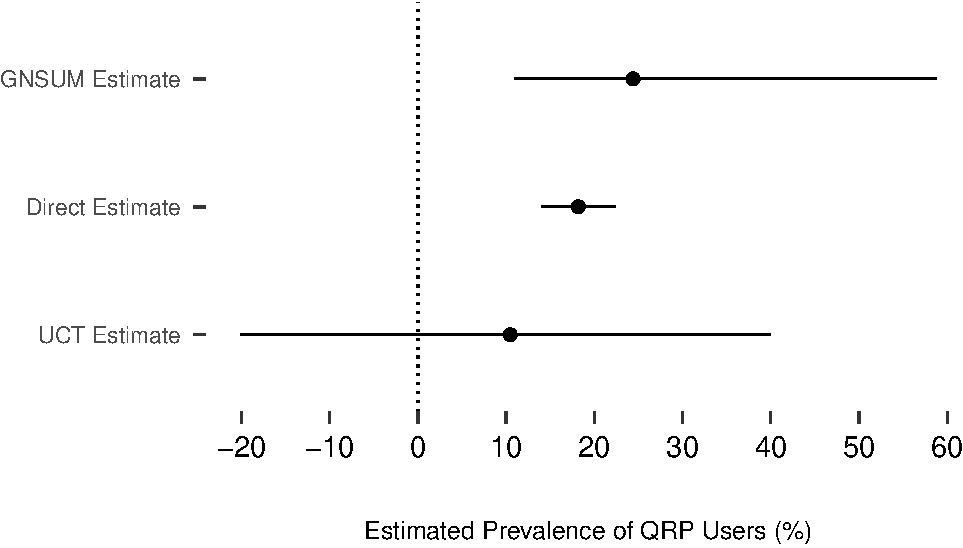
\includegraphics{How_Many_QRP_Users_preprint_files/figure-latex/unnamed-chunk-13-1.pdf}
\caption{\label{fig:unnamed-chunk-13}\label{fig:estimate}Estimates of the
current prevalence of users of questionable research practices using
three different estimators; the Generalized Network Scale-Up Method
(GNSUM), the Direct Estimate, and the Unmatched Count Technique (UCT).
Point estimates with 95\% bootstrapped confidence intervals.}
\end{figure}

\subsection{Direct Estimate}\label{direct-estimate-1}

To ensure the highest number of participants in our game of contacts,
half of the total population were asked to participate in Survey 3,
which contained our direct estimate question. Thus, 3,551 psychologists
were solicited, and we received 308 responses to Survey 3 able to be
analyzed. Of the 308 participants, 56 indicated they had used at least
one QRP in the past 12 months. Using Equation 1, we calculated QRP
prevalence to be 18.18\% (bootstrapped 95\% confidence interval
{[}13.96\%, 22.40\%{]}). This corresponds to an estimated 1,291 American
psychologists currently using QRPs.

It is possible this estimate underestimates the true number of
psychologists using QRPs. For one, social desirability may lead some
scientists who have used QRPs to be unwilling to admit it. This estimate
is only generated by those participants willing to reveal their identity
as a QRP user. Given the somewhat critical social environment for QRP
users (Fiske, 2016; Teixeira da Silva, 2018), it is reasonable to
believe some participants withheld their identity when we asked
directly. The following indirect estimation methods sought to mitigate
this social desirability bias.

\subsection{Unmatched Count
Technique}\label{unmatched-count-technique-1}

The remaining 3,550 psychologists contacted were asked to participate in
our unmatched count estimate with 1,775 randomized into the innocuous
list condition, and 1,775 randomized into the sensitive list condition.
From this, we received 279 responses for analysis.

The average number of list items corresponding to participants in the
innocuous list condition was 4.28. The average number of list items
corresponding to participants in the sensitive list condition was 4.39.
Using Equation 2, we calculated QRP user prevalence to be 10.46\%
{[}-20.19\%, 22.40\%{]}. This corresponds to an estimated 743 American
psychologists currently using QRPs.

It was unexpected that the calculated UCT estimate would be lower than
our direct estimate. Typically, due to reducing response bias, UCT
estimates are larger than direct estimates when the behavior or identity
in question is concealable and potentially stigmatized (Gervais \&
Najle, 2017; Starosta \& Earleywine, 2014; Wolter \& Laier, 2014). Given
the bootstrapped 95\% confidence interval crosses zero, it is likely the
relatively low number of participants in our UCT (n = 279) led this
calculation to be overly sensitive to individual responses, and as such,
we do not consider this estimate to be valid or accurate.

\subsection{Generalized Network Scale-Up
Estimate}\label{generalized-network-scale-up-estimate}

All participants who were randomized into the UCT estimate were also
asked to answer questions about their social networks, and to estimate
how many researchers they know who have used at least one QRP in the
past 12 months. Participants who were randomized into the direct
estimate and who self-identified as a QRP user in that estimate were
also asked to answer questions about their social network and to
participate in the game of contacts method. Participants in the direct
estimate who did not self-identify as a QRP user were asked questions
about their social network as well, but were not asked how many
researchers they know who have used at least one QRP in the past 12
months. Therefore, we collected social network responses from 531
participants from the general frame population (to be used in estimating
\(\delta\)), 56 responses from participants who self-identified as QRP
users who also completed the game of contacts (to be used in estimating
\(\tau\) and \(\delta\)), and 279 responses from participants who
estimated the number of researchers they know who have used at least one
QRP in the past 12 months.

These 279 individuals identified a sum total of 664 QRP users, and know
a sum total of 46,828 researchers. Given the total frame population is
7,101, we are fairly confident all or nearly all members were identified
at least once by our participants. Using the network scale-up in
Equation 3, this generates an estimate of 1.42\% {[}0.85\%, 2.14\%{]}.
This estimate serves as the base starting point our key network
estimate, the Generalized Network Scale-Up Estimator (GNSUM), detailed
below.

Equation 5 relaxes the assumptions of equal network size and total
information transmission by incorporating \(\tau\) and \(\delta\). Using
the 531 responses from the general population and the 56 responses from
the participants who indicated using a QRP in the past 12 months, we
estimate \(\delta\) as 0.97. Using the game of contacts, we estimate
\(\tau\) as 0.06. Using Equation 5, we estimate QRP user prevalence to
be 24.40\% {[}10.93\%, 58.74\%{]}. This corresponds to an estimated
1,733 American psychologists currently using QRPs.

Additional analyses assessed the validity of the GNSUM in this
population by using it to generate estimates of other populations of
known size. GNSUM estimates were then compared to those actual
population sizes. If GNSUM estimates correspond well with the actual
size of these populations, it would suggest that the GNSUM most likely
provides a good estimate of population size in this group of
participants.

To this end, we generated additional estimates of 24 populations of
known size; the number of psychologists with particular first names (the
number of psychologists named David, named Janet, etc). The 24 names
were gender balanced and represented common, uncommon, and rare names
that exist within the census of the population of interest. The size
estimates of these populations of known size can be seen in Figure
\ref{fig:validity}. The estimates made by our participants of the size
of these 24 populations closely mirror the actual prevalence of these
groups. The correlation between our participant's estimate of those
group sizes and the actual group sizes is r = 0.91. We cannot know for
certain whether the GNSUM estimate accurately identified the proportion
of QRP users in psychology. Nonetheless, that using the GNSUM with these
same participants accurately estimated the size of multiple known
populations is consistent with the conclusion that our GNSUM estimate
also accurately estimates the proportion of QRP users in psychology.

\begin{figure}
\centering
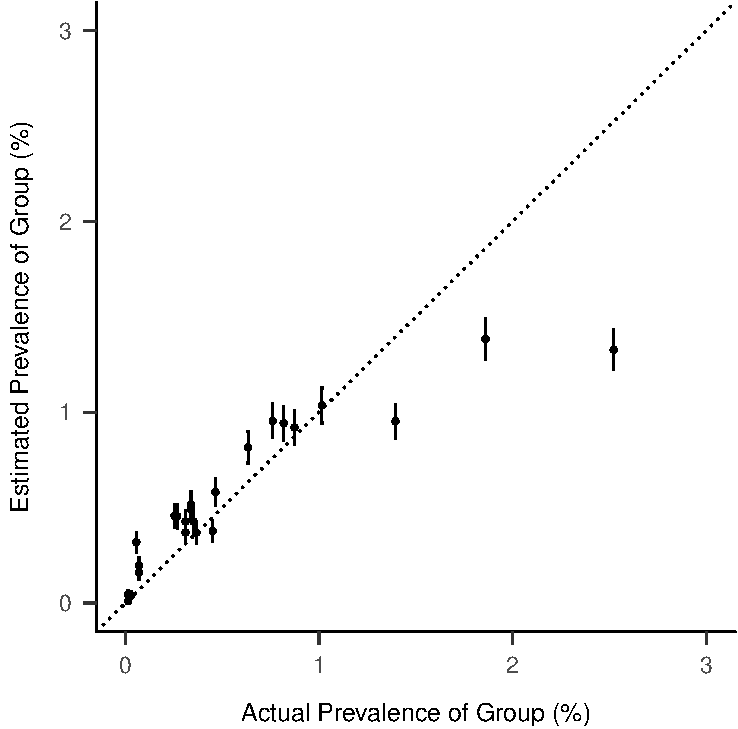
\includegraphics{How_Many_QRP_Users_preprint_files/figure-latex/unnamed-chunk-14-1.pdf}
\caption{\label{fig:unnamed-chunk-14}\label{fig:validity}Validation of
Network Scale-Up Estimates using 24 groups of known size. Each point
represents one group, with 95\% confidence intervals. Dotted line
represents when estimated group prevalence equals actual group
prevalence. Correlation between estimated and actual group prevalence, r
= 0.91.}
\end{figure}

\section{DISCUSSION}\label{discussion}

Because of inconsistencies in previous research, this study generated
three estimates of current QRP use, using three independent estimating
procedures. Depending on the estimator used, we estimate 18.18\% to
24.40\% of American psychologists currently use questionable research
practices. Our unmatched count estimate produced an estimate of 10.46\%,
though this may not be a valid or accurate estimate.

To the best of our knowledge, this is the first report of the prevalence
of QRP users in a proximal timespan. As such, it is difficult to draw
conclusions about the magnitude of our estimates when compared to
previous estimates.

Compared to John et al. (2012) and Agnoli et al. (2017), we estimate
lower rates of questionable research practices. Compared to Fiedler and
Schwarz (2016), however, we estimate higher rates of these practices.
Our definition of \enquote{questionable research practices} were the
same ones used in John et al. (2012) and Agnoli et al. (2017), but was
restricted to a timespan of only 15 months, so it is reasonable that our
estimates would be lower than those with an unrestricted timeframe of
QRP use. Since we used those same QRP definitions, is also reasonable
that our estimates would be higher than those described by Fiedler and
Schwarz (2016), who changed the definitions of each QRP.

This is also the first report to use the generalized network-scale up
estimator to investigate the prevalence of QRP users in psychology.
Direct estimates rely on an individual's willingness to participate and
their willingness to honestly share their identity as a QRP user. Bias
in either of these dimensions can distort a direct estimate.

Social network methods, on the other hand, enable researchers to better
understand the social processes at work that produce an environment
where members vary in their identity and the information they share with
others (Zheng et al., 2006). In the process of producing a population
size estimate for current QRP users, we also reported the first estimate
of the social transmission of this QRP-use identity - tau (\(\tau\)), of
0.06, or 6.02\%.

\subsection{Implications}\label{implications}

These estimates serve as a baseline to measure the effectiveness of
current initiatives, as well as a foundation for new ones. While much
work is being done to grow support for interventions such as
pre-registration (E.-J. Wagenmakers \& Dutilh, 2016) and Registered
Reports (D. Chambers, Feredoes, D. Muthukumaraswamy, \& J. Etchells,
2014), it is currently unknown what quantitative effect these are having
on curbing behaviors associated with inflated Type I error such as QRPs.
By performing follow-up estimates at future time points, the field can
use the baseline estimates presented here to measure the effectiveness
of these programs at reducing QRP use.

\subsection{Limitations \& Future
Directions}\label{limitations-future-directions}

Our unmatched count estimate was lower than our direct estimate and had
a confidence interval that included zero, which we did not expect. This
estimate is computed as a difference between averages, which means each
is sensitive to the number of participants. Our innocuous item group had
130 participants, and our concealable item group had 149 participants.
As denominators in computing the means needed for Equation 2, these are
low. For example, if one additional participant in the innocuous list
condition responded by itentifying with 6 of 9 items (1 standard
deviation above the mean), our UCT estimate would change from 10.46\% to
9.15\%. This is reflected in the bootstrapped confidence interval
crossing zero, indicative of an unstable difference between the
innocuous and concealable list groups. Future work using the UCT would
benefit from larger sample sizes, as demonstrated in Gervais and Najle
(2017).

As noted in the introduction, QRPs exist in a grey area of accepted
scientific practice. Therefore, it is difficult to interpret the
severity of QRP use. This difficulty, along with the high variability
among previous estimates of QRP prevalence, has led to a number of
different conclusions. Some have concluded that the problems are
overstated (Fanelli, 2018), while others argue QRP use presents a real
threat to the viability of several scientific fields, such as education
and political science (Bosco, Aguinis, Field, Pierce, \& Dalton, 2016).
Although our work moves the field forward in understanding the
prevalence of those that use these behaviors, it provides less guidance
on the severity of the consequences of QRP use on the whole.

Science is a globally distributed network, and as such, can be difficult
to study. Our reported estimates were limited to American psychologists,
though we know that these issues are not restricted solely to the United
States (Agnoli et al., 2017; Fiedler \& Schwarz, 2016; Forsberg et al.,
2018). Future studies estimating the prevalence of QRP use in other
countries will be an important next step, as will investigating the use
of QRPs in other scientific fields. Some of this work has already
started through the Horizon 2020 framework in the European Union
(Forsberg et al., 2018), though more innovative work will be required to
better understand the scope of the problems faced.

\subsection{Conclusion}\label{conclusion}

By directly asking participants about their use of QRPs, we estimate
18.18\% have used at least one QRP in the past 12 months. The
generalized network scale up estimate is 24.40\%, which corresponds to
between 1,291 and 1,733 American psychologists. Although some have
argued the narrative of the \enquote{replication crisis} is overblown
(Fanelli, 2018), the current work illustrates how common QRP use is.
Although many have called for changes in statistical inference practices
to mitigate false-positive findings (Benjamin et al., 2017; Lakens et
al., 2018; Mcshane, Gal, Gelman, Robert, \& Tackett, 2017), it is
important that we as a field also focus on disincentivizing the use of
questionable research practices (and other behavioral degrees of
freedom) among our peers and coworkers for the betterment of our
science.

\newpage

\section{References}\label{references}

\begingroup
\setlength{\parindent}{-0.5in} \setlength{\leftskip}{0.5in}

\hypertarget{refs}{}
\hypertarget{ref-Agnoli2017}{}
Agnoli, F., Wicherts, J. M., Veldkamp, C. L. S., Albiero, P., \&
Cubelli, R. (2017). Questionable research practices among Italian
research psychologists. \emph{PLoS ONE}, \emph{12}(3), 1--17.
doi:\href{https://doi.org/10.1371/journal.pone.0172792}{10.1371/journal.pone.0172792}

\hypertarget{ref-Ahrnsbrak2017}{}
Ahrnsbrak, R., Bose, J., Hedden, S., Lipari, R., \& Park-Lee, E. (2017).
Key Substance Use and Mental Health Indicators in the United States:
Results from the 2016 National Survey on Drug Use and Health.
\emph{Substance Abuse and Mental Health Services Administration},
\emph{7}(1), 877--726.
doi:\href{https://doi.org/10.1016/j.drugalcdep.2016.10.042}{10.1016/j.drugalcdep.2016.10.042}

\hypertarget{ref-Arentoft2016}{}
Arentoft, A., Van Dyk, K., Thames, A. D., Sayegh, P., Thaler, N.,
Schonfeld, D., \ldots{} Hinkin, C. H. (2016). Comparing the unmatched
count technique and direct self-report for sensitive health-risk
behaviors in HIV+ adults. \emph{AIDS Care - Psychological and
Socio-Medical Aspects of AIDS/HIV}, \emph{28}(3), 370--375.
doi:\href{https://doi.org/10.1080/09540121.2015.1090538}{10.1080/09540121.2015.1090538}

\hypertarget{ref-Benjamin2017}{}
Benjamin, D. J., Berger, J. O., Johannesson, M., Nosek, B. A.,
Wagenmakers, E. J., Berk, R., \& Johnson, V. E. (2017). Redefine
Statistical Significance. \emph{PsyArxiv}, (July 22), 1--18.
doi:\href{https://doi.org/10.17605/OSF.IO/MKY9J}{10.17605/OSF.IO/MKY9J}

\hypertarget{ref-Bernard2010}{}
Bernard, H. R., Hallett, T., Iovita, A., Johnsen, E. C., Lyerla, R.,
McCarty, C., \ldots{} Stroup, D. F. (2010). Counting hard-to-count
populations: the network scale-up method for public health.
\emph{Sexually Transmitted Infections}, \emph{86 Suppl 2}, ii11--5.
doi:\href{https://doi.org/10.1136/sti.2010.044446}{10.1136/sti.2010.044446}

\hypertarget{ref-Bosco2016}{}
Bosco, F. A., Aguinis, H., Field, J. G., Pierce, C. A., \& Dalton, D. R.
(2016). HARKing's Threat to Organizational Research: Evidence From
Primary and Meta-Analytic Sources. \emph{Personnel Psychology},
\emph{69}(3), 709--750.
doi:\href{https://doi.org/10.1111/peps.12111}{10.1111/peps.12111}

\hypertarget{ref-Button2013}{}
Button, K. S., Ioannidis, J. P. A., Mokrysz, C., Nosek, B. A., Flint,
J., Robinson, E. S. J., \& Munafò, M. R. (2013). Power failure: why
small sample size undermines the reliability of neuroscience.
\emph{Nature Reviews Neuroscience}, \emph{14}(5), 365--376.
doi:\href{https://doi.org/10.1038/nrn3475}{10.1038/nrn3475}

\hypertarget{ref-Connelly1995}{}
Connelly, N. A., \& Brown, T. L. (1995). Use of Angler Diaries to
Examine Biases Associated with 12-Month Recall on Mail Questionnaires.
\emph{Transactions of the American Fisheries Society}, \emph{124}(3),
413--422.
doi:\href{https://doi.org/10.1577/1548-8659(1995)124\%3C0413:uoadte\%3E2.3.co;2}{10.1577/1548-8659(1995)124\textless{}0413:uoadte\textgreater{}2.3.co;2}

\hypertarget{ref-Chambers2014}{}
D. Chambers, C., Feredoes, E., D. Muthukumaraswamy, S., \& J. Etchells,
P. (2014). Instead of ``playing the game'' it is time to change the
rules: Registered Reports at AIMS Neuroscience and beyond. \emph{AIMS
Neuroscience}, \emph{1}(1), 4--17.
doi:\href{https://doi.org/10.3934/Neuroscience.2014.1.4}{10.3934/Neuroscience.2014.1.4}

\hypertarget{ref-Fanelli2018}{}
Fanelli, D. (2018). Is science really facing a reproducibility crisis,
and do we need it to? \emph{Proceedings of the National Academy of
Sciences of the United States of America2}, \emph{in press}, 1--4.
doi:\href{https://doi.org/10.1073/pnas.1708272114}{10.1073/pnas.1708272114}

\hypertarget{ref-Fiedler2016}{}
Fiedler, K., \& Schwarz, N. (2016). Questionable Research Practices
Revisited. \emph{Social Psychological and Personality Science},
\emph{7}(1), 45--52.
doi:\href{https://doi.org/10.1177/1948550615612150}{10.1177/1948550615612150}

\hypertarget{ref-Fiske2016}{}
Fiske, S. T. (2016). Mob Rule or Wisdom of Crowds. \emph{APS Observer}.

\hypertarget{ref-Forsberg2018}{}
Forsberg, E. M., Anthun, F. O., Bailey, S., Birchley, G., Bout, H.,
Casonato, C., \ldots{} Zöller, M. (2018). Working with Research
Integrity---Guidance for Research Performing Organisations: The Bonn
PRINTEGER Statement. \emph{Science and Engineering Ethics}, 1--12.
doi:\href{https://doi.org/10.1007/s11948-018-0034-4}{10.1007/s11948-018-0034-4}

\hypertarget{ref-Gervais2017}{}
Gervais, W. M., \& Najle, M. B. (2017). How many atheists are there?
\emph{Social Psychological and Personality Science}, 1948550617707015.

\hypertarget{ref-Jing2014}{}
Jing, L., Qu, C., Yu, H., Wang, T., \& Cui, Y. (2014). Estimating the
sizes of populations at high risk for HIV: A comparison study.
\emph{PLoS ONE}, \emph{9}(4), 1--6.
doi:\href{https://doi.org/10.1371/journal.pone.0095601}{10.1371/journal.pone.0095601}

\hypertarget{ref-John2012}{}
John, L. K., Loewenstein, G., \& Prelec, D. (2012). Measuring the
Prevalence of Questionable Research Practices With Incentives for Truth
Telling. \emph{Psychological Science}, \emph{23}(5), 524--532.
doi:\href{https://doi.org/10.1177/0956797611430953}{10.1177/0956797611430953}

\hypertarget{ref-Killworth1998a}{}
Killworth, P., McCarty, C., Bernard, H. R., Shelley, G. A., \& Johnsen,
E. C. (1998). Estimation of Seroprevalence, Rape, and Homelessness in
the U.S. Using a Social Network Approach. \emph{Evaluation Review},
\emph{22}, 289--308.

\hypertarget{ref-Lakensabc1860}{}
Lakens, D., Adolfi, F. G., Albers, C. J., Anvari, F., J Apps, M. A.,
Argamon, S. E., \ldots{} Lino de Oliveira, C. (2018). Justify Your
Alpha: A Response to `` Redefine Statistical Significance''.
\emph{Nature Human Behavior}, \emph{2}, 168--171.

\hypertarget{ref-Landen1995}{}
Landen, D. D., \& Hendricks, S. (1995). Effect of recall on reporting of
at-work injuries. \emph{Public Health Reports (Washington, D.C. :
1974)}, \emph{110}(3), 350--4.
doi:\href{https://doi.org/10.1016/s0022-4375(97)90342-x}{10.1016/s0022-4375(97)90342-x}

\hypertarget{ref-McCormick2010}{}
McCormick, T. H., Salganik, M. J., \& Zheng, T. (2010). How many people
do you know? Efficiently estimating personal network size. \emph{J Am
Stat Assoc.}, \emph{105}(489), 59--70.
doi:\href{https://doi.org/10.1016/j.immuni.2010.12.017.Two-stage}{10.1016/j.immuni.2010.12.017.Two-stage}

\hypertarget{ref-Mcshane2017}{}
Mcshane, B. B., Gal, D., Gelman, A., Robert, C., \& Tackett, J. L.
(2017). Abandon Statistical Significance, 1--12.

\hypertarget{ref-Qualtrics}{}
Qualtrics. (2005). Qualtrics Survey Software. Retrieved from
\url{www.qualtrics.com}

\hypertarget{ref-Salganik2011}{}
Salganik, M. J., Fazito, D., Bertoni, N., Abdo, A. H., Mello, M. B., \&
Bastos, F. I. (2011). Assessing network scale-up estimates for groups
most at risk of HIV/AIDS: Evidence from a multiple-method study of heavy
drug users in Curitiba, Brazil. \emph{American Journal of Epidemiology},
\emph{174}(10), 1190--1196.
doi:\href{https://doi.org/10.1093/aje/kwr246}{10.1093/aje/kwr246}

\hypertarget{ref-Salganik2012}{}
Salganik, M. J., Mello, M., Abdo, A., Bertoni, N., Fazito, D., \&
Bastos, F. (2012). The Game of Contacts: Estimating the Social
Visibility of Groups, \emph{100}(2), 130--134.
doi:\href{https://doi.org/10.1016/j.pestbp.2011.02.012.Investigations}{10.1016/j.pestbp.2011.02.012.Investigations}

\hypertarget{ref-Simmons2011}{}
Simmons, J. P., Nelson, L. D., \& Simonsohn, U. (2011). False-Positive
Psychology. \emph{Psychological Science}, \emph{22}(11), 1359--1366.
doi:\href{https://doi.org/10.1177/0956797611417632}{10.1177/0956797611417632}

\hypertarget{ref-Starosta2014}{}
Starosta, A. J., \& Earleywine, M. (2014). Assessing base rates of
sexual behavior using the unmatched count technique. \emph{Health
Psychology and Behavioral Medicine}, \emph{2}(1), 198--210.
doi:\href{https://doi.org/10.1080/21642850.2014.886957}{10.1080/21642850.2014.886957}

\hypertarget{ref-TeixeiradaSilva2018}{}
Teixeira da Silva, J. A. (2018). Freedom of Speech and Public Shaming by
the Science Watchdogs. \emph{Journal of Advocacy, Research, and
Education}, \emph{5}(1).

\hypertarget{ref-NHIS2006}{}
United States Census Bureau. (2018). \emph{National health Interview
Survey: CAPI Manual for NHIS Field Representative} (No. January).
Retrieved from
\href{ftp://ftp.cdc.gov/pub/health\%7B/_\%7Dstatistics/nchs/Survey\%7B/_\%7DQuestionnaires/NHIS/2006/frmanual.pdf}{ftp://ftp.cdc.gov/pub/health\{\textbackslash{}\_\}statistics/nchs/Survey\{\textbackslash{}\_\}Questionnaires/NHIS/2006/frmanual.pdf}

\hypertarget{ref-Wagenmakers2016}{}
Wagenmakers, E.-J., \& Dutilh, G. (2016). Seven Selfish Reasons for
Preregistration. Retrieved from
\url{https://www.psychologicalscience.org/observer/seven-selfish-reasons-for-preregistration/comment-page-1}

\hypertarget{ref-Wicherts2016}{}
Wicherts, J. M., Veldkamp, C. L., Augusteijn, H. E., Bakker, M., Aert,
R. C. van, \& Assen, M. A. van. (2016). Degrees of freedom in planning,
running, analyzing, and reporting psychological studies: A checklist to
avoid P-hacking. \emph{Frontiers in Psychology}, \emph{7}(NOV), 1--12.
doi:\href{https://doi.org/10.3389/fpsyg.2016.01832}{10.3389/fpsyg.2016.01832}

\hypertarget{ref-Wolter2014}{}
Wolter, F., \& Laier, B. (2014). The Effectiveness of the Item Count
Technique in Eliciting Valid Answers to Sensitive Questions. An
Evaluation in the Context of Self-Reported Delinquency. \emph{Survey
Research Methods}, \emph{8}(3), 153--168.

\hypertarget{ref-Zhang2010}{}
Zhang, T. Y., Hellstrom, I. C., Bagot, R. C., Wen, X., Diorio, J., \&
Meaney, M. J. (2010). Maternal care and DNA methylation of a glutamic
acid decarboxylase 1 promoter in rat hippocampus. \emph{J Neurosci},
\emph{30}(39), 13130--13137.
doi:\href{https://doi.org/10.1523/JNEUROSCI.1039-10.2010}{10.1523/JNEUROSCI.1039-10.2010}

\hypertarget{ref-Zheng2006}{}
Zheng, T., Salganik, M. J., \& Gelman, A. (2006). How Many People Do You
Know in Prison? \emph{Journal of the American Statistical Association},
\emph{101}(474), 409--423.
doi:\href{https://doi.org/10.1198/016214505000001168}{10.1198/016214505000001168}

\endgroup


\end{document}
